% generated by plots/fig6_violence.py --- do not edit the numbers by hand
% figure* --- the chapter is two-column and this does not fit one
\begin{figure*}[tp]
\centering
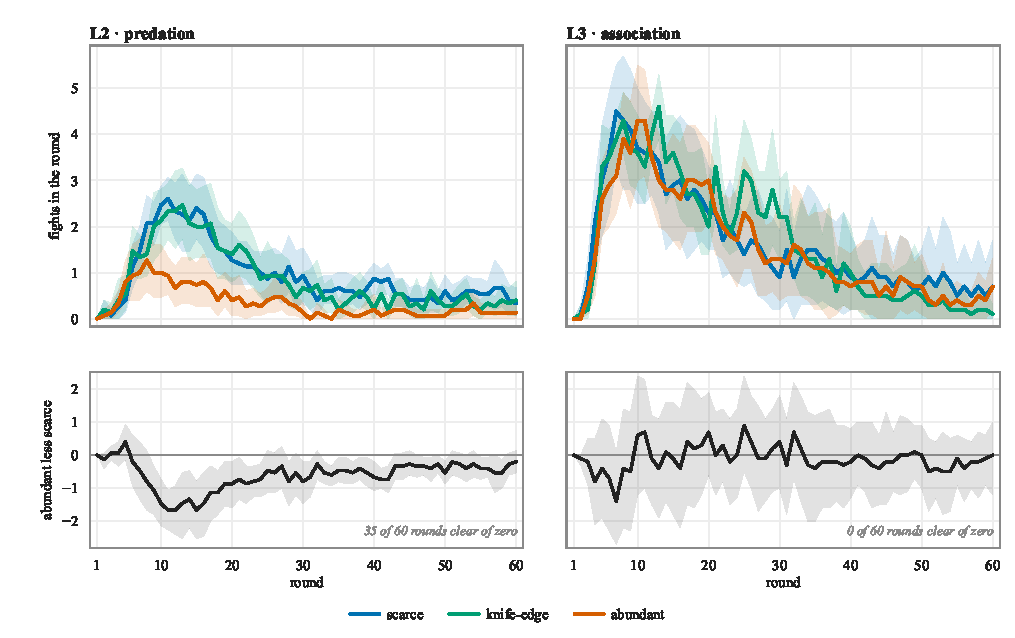
\includegraphics[width=\linewidth]{figures/fig6_violence/over_time.pdf}\\[2pt]
\caption[When the fighting happens]{%
\textbf{When the fighting happens.} Fights per round against the round they fell in. Above, the cell mean as a line with a 95 per cent interval over runs, fifteen runs per cell at L2 and ten at L3. Below, the abundant cell less the scarce one, with an interval on the difference itself and a line at zero: two bands that overlap can still have a difference clear of zero, so the lower row is the test and the upper row the shape. L1 and L4 are not drawn, since no run at either level resolves more than two fights in the whole game.}
\label{fig:violence}
\end{figure*}
